
\def \Subject {گزارش پروژه}
\def \Course {درس امنیت سیستم های کامپیوتری}
\def \Author {نیما کمبرانی, فاطمه زهرا بخشنده}
\def \Report {مینی پروژه 2}
\def \StudentNumber {98521423 , 98522157}

\begin{center}
\vspace{.4cm}
{\bf {\huge \Subject}}\\
\vspace{.5cm}
{\bf \Large \Course}
\vspace{.2cm}
\end{center}
{\bf \Author }  \\
{\bf شماره دانشجویی:\ \StudentNumber}
\hspace{\fill} 
{\Large \Report} \\
\hrule
\vspace{0.8cm}

\clearpage

%\huge{\Subject}\\[1.5 cm]
%\chapterauthor{\Author~ : \StudentNumber}
\par

\section{سوال 1}
\subsection{توضیحات}
\paragraph{}
حمله تفاضلی در سال 1990 بر روی الگوریتم 
\lr{DES}
ارائه داده شد. این روش با این فرض کار می‌کند که با داشتن دو یا چند متن اولیه و متن رمز شده متناظر آن‌ها و بدست آوردن تفاضل هر یک از جفت متن‌ها و متن رمزشده  متناظر آن‌ها ممکن است رابطه‌ای بین ریاضی بین تفاضل در متن اولیه و متن رمز وجود داشته باشد که با توجه به آن بتوان کل یا تعدادی از بیت های کلید را بدست آورد. درنتیجه با بدست آوردن برخی بیت های کلید شکستن کامل آن در زمان کمتری انجام خواهد شد و امنیت الگوریتم رمزنگاری از بین می‌رود. این روش می‌تواند با استفاده از روش های شکستن رمز  متن رمز انتخابی
(
\lr{chosen cipher text attack}
) 
یا متن اولیه انتخابی 
(
\lr{chosen plaintext attack}
)
اجرا شوند. 
\paragraph{}
در صورتی که الگوریتم نسبت به این نوع حمله  مقاوم نباشد، می‌توان آن را با داشتن تعداد کمی متن ساده و متن رمز متناظر آن‌ها با سرعت بسیار بیشتر نسبت به 
\lr{Brute force}
اقدام به شکستن رمز کنیم. به عنوان مثال در الگوریتم 
\lr{FEAL-4} 
می‌توان تنها با داشتن 8 جفت متن ساده انتخاب شده به سادگی الگوریتم را شکست.

\paragraph{}
برای انجام این حمله به صورت 
\lr{chosen plaintext}
، ابتدا تعدادی جفت متن ورودی انتخاب می‌کنیم. متن های انتخاب شده باید یک اختلاف ثابت داشته باشند، مثلا همه آن‌ها در بیت 5 ام اختلاف داشته باشند. پس از ساختن تعدادی جفت متن آشکار هر یک از متن‌ها با استفاده از کلید یکسان رمز می‌شوند. پس از رمزگذاری، اختلاف متن‌های رمز شده را نیز بدست می‌آوریم. پس از یافتن اختلاف متن‌های رمز شده با استفاده از تحلیل آماری به دنبال نشانه های از عدم وجود رابطه تصادفی در بین اختلاف متن رمز شده و متن اشکار می‌گردیم. بعنوان مثال اگر درصد زیادی از متن های رمز شده در یک بیت خاص تفاوت داشته باشند یا اختلاف یکسانی داشته باشند نشان از وجود رابطه بین تغییرات در متن اشکار و متن رمز شده است. در نتیجه با استفاده از این دانش می‌توان تعدادی از بیت های کلید را به دست آورد و عملیات شکستن کامل کلید را در زمان کمتری انجام داد.

\paragraph{}
همچنین برای انجام این حمله بصورت 
\lr{chosen ciphertext}
بصورت مشابه تعدادی متن رمز با اختلاف ثابت می‌سازیم و با بررسی روابط آماری در متن آشکار متناظر، 
به دنبال شواهد وجود الگو ها و روابط غیر تصادفی می‌گردیم.


مثال با 
\lr{DES}
سه دور:
فرض کنید که می‌خواهیم یک پیام رمزنگاری شده با الگوریتم 
\lr{DES}
 سه دوره رمزگشایی کنیم. اگر برای  رمزنگاری این پیام از کلید
\lr{0123456789ABCDEF}
 استفاده شود.
سپس برای رمزنگاری پیام، از مراحل زیر عبور می‌کنیم:

مرحله ۱: اعمال تابع اولیه با ترکیب کلید و بلاک اول پیام

مرحله ۲: ۳ دور اعمال تابع‌های 
\lr{F}
و تابع جعبه جایگشتی

مرحله ۳: اعمال تابع اختصاصی با استفاده از کلید و بلاک آخر پیام

اگر پیام زیر را با کلید بالا رمزنگاری کنیم
و پس از رمزنگاری، خروجی زیر را دریافت کنیم:
\lr{85E813540F0AB405}

حال با فرض یک تفاوت یک بیتی بین ورودی‌های رمزنگاری، مثلاً بین پیام اصلی و پیامی که یک بیت آخر آن تغییر کرده است، با داشتن خروجی رمزنگاری این دو ورودی رمزنگاری را انجام داده و تفاوت خروجی را محاسبه می‌کنیم. اگر تفاوت خروجی برابر با یک الفبای ۱۶
بیتی باشد، احتمال دارد که برخی اجزای الگوریتم رمزنگاری به یک شکل خاصی وابسته باشند و این ممکن است راهی برای برداشتن اطلاعات درباره الگوریتم باشد. این نوع حمله در طی چندین مرحله و با تلاش مکرر برای پیدا کردن تفاوت‌های دیگر، به محاسبه‌ی کلید استفاده شده در رمزنگاری پیام کمک می‌کند.

با توجه به شدت حملات تفاضلی بر روی 
\lr{DES}
، استفاده از این الگوریتم به عنوان یک الگوریتم رمزنگاری امن، امروزه توصیه نمی‌شود و به جای آن، الگوریتم‌های قوی‌تر و امن‌تری مانند 
/lr{AES}
پیشنهاد می‌شوند.


\section{سوال 2}

\subsection{الگوریتم \lr{AES}}

\paragraph{}
الگوریتم 
\lr{AES}
یک الگوریتم رمزنگاری متقارن از نوع 
\lr{Block cipher}
است که در بسیاری از کاربرد های نیازمند به رمز نگاری کاربرد دارد. این الگوریتم دارای طول کلید های 128، 196 و 256 بیت برای است که هرچه طول کلید آن بلندتر باشد امنیت بالاتری دارد.
این الگوریتم در هرمرتبه از 4 عملگر اصلی برای رمز نگاری استفاده می‌کند. در ابتدا متن ورودی به بلاک های با طول 128 بیت (16 بایت) تقسیم می‌کند. سپس بلاک 16 بایتی بدست آمده را به صورت یک ماتریس 4*4 در می‌آورد سپس مراحل رمز نگاری بر روی آن انجام می‌شود.


مراحل بصورت زیر هستند:
\subsubsection{مراحل}

\begin{figure}[h!]
    \centering
    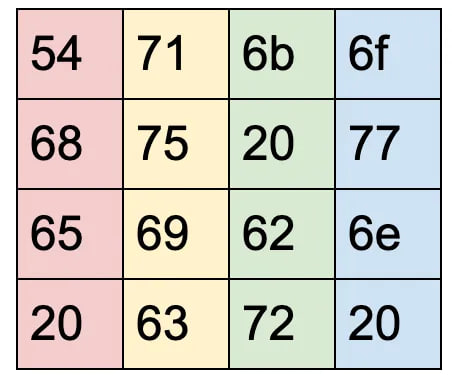
\includegraphics[width=0.5\linewidth]{images/initial text.jpg}
    \caption{متن آشکار اولیه که یک بخش 128 بیت از آن بصورت ماتریس 4 در 4 تبدیل شده است
    }
    \label{fig:init}
\end{figure}

\begin{figure}[h!]
    \centering
    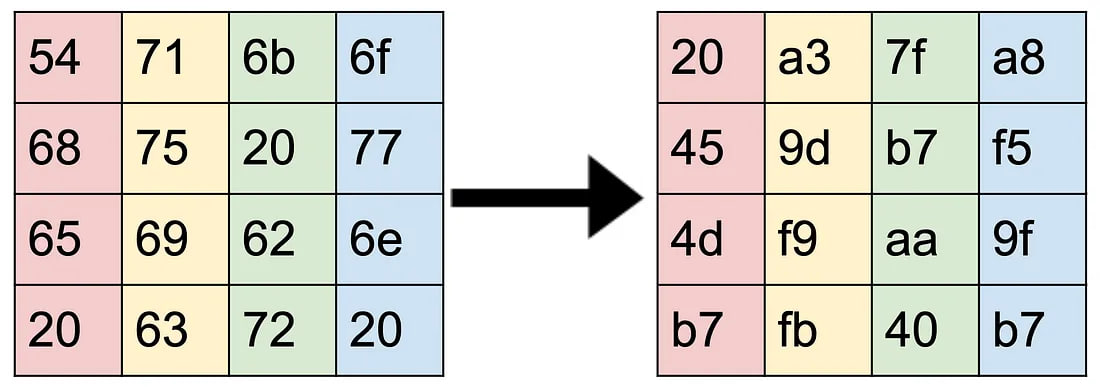
\includegraphics[width=0.5\linewidth]{images/apply_sbox.jpg}
    \caption{اعمال تابع غیرخطی\lr{sbox} بر روی هر یک از بایت های متن}
    \label{fig:addsbox}
\end{figure}

\begin{figure}[h!]
    \centering
    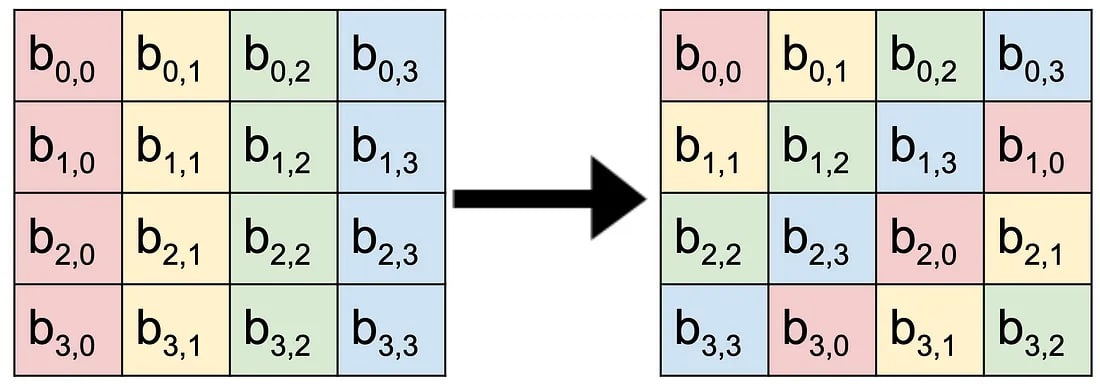
\includegraphics[width=0.5\linewidth]{images/Shift rows.jpg}
    \caption{جابه‌جا کردن و شیفت دادن ردیف ها }
    \label{fig:addshift}
\end{figure}

\begin{figure}[h!]
    \centering
    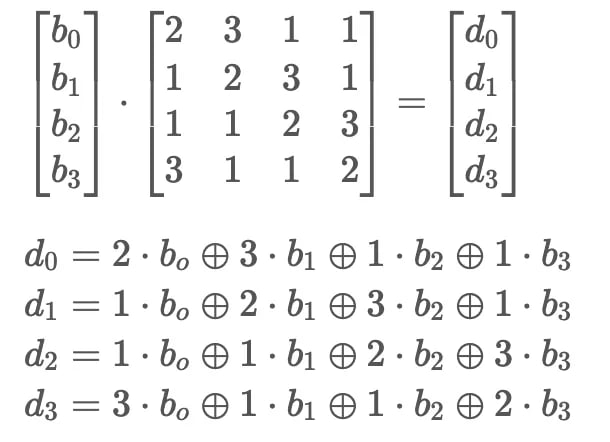
\includegraphics[width=0.5\linewidth]{images/transformation.jpg}
    \caption{تبدیل ماتریس اعمال شده در هر مرحله بر روی هر ستون از متن}
    \label{fig:transform}
\end{figure}

\begin{figure}[h!]
    \centering
    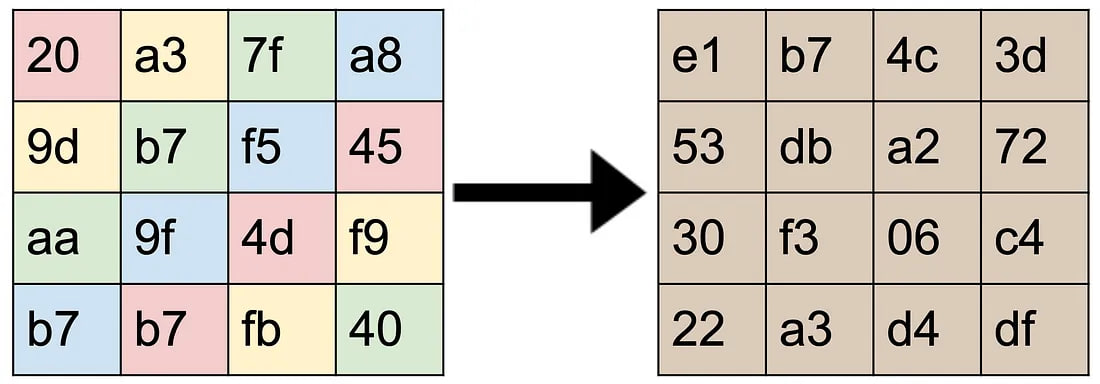
\includegraphics[width=0.5\linewidth]{images/add transformation.jpg}
    \caption{اعمال تبدیل ماتریسی بر روی متن برای ترکیب کردن ستون ها}
    \label{fig:addtransfor}
\end{figure}

\begin{figure}[h!]
    \centering
    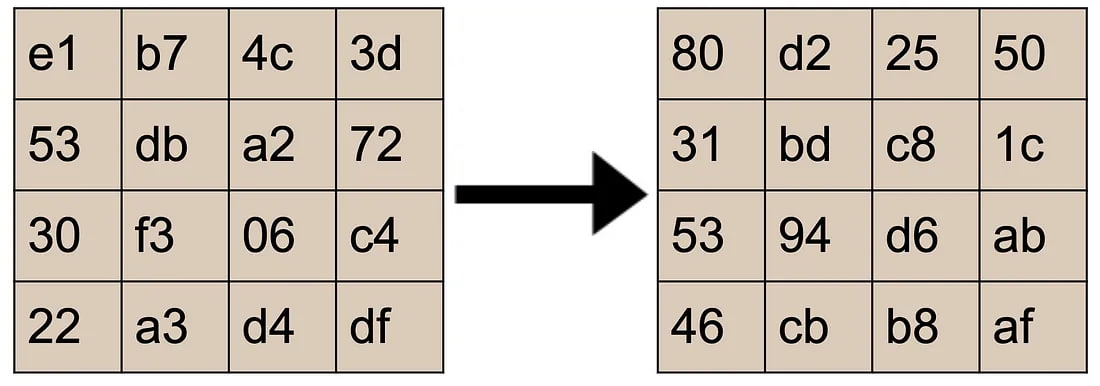
\includegraphics[width=0.5\linewidth]{images/add_key.jpg}
    \caption{ترکیب متن با کلید بصورت عملیات xor}
    \label{fig:addkey}
\end{figure}
\newpage

\subsection{نمونه}
\begin{figure}[h!]
    \centering
    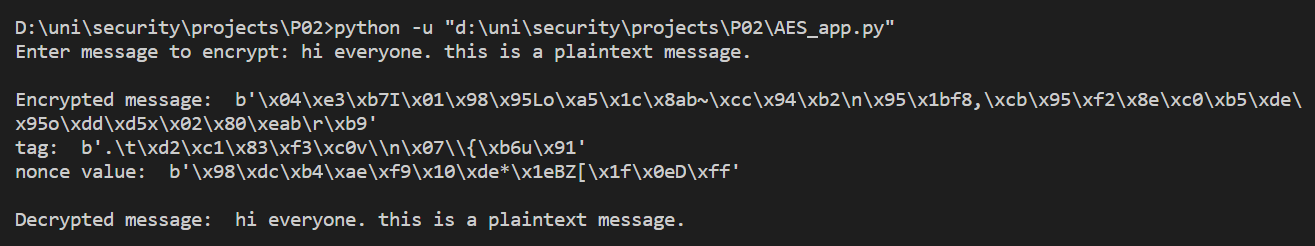
\includegraphics[width=0.9\linewidth]{images/AES.png}
    \caption{خروجی کنسول برای رمزنگاری و رمزگشایی یک پیام}
    \label{fig:addkey}
\end{figure}

\subsection{کد سوال}
 کد سوال با استفاده از زبان پایتون پیاده شده، و از کتابخانه
  \lr{pycryptodome}
 در آن استفاده است. 
 
 در این برنامه با گرفتن یک پیام از کاربر ابتدا آن را رمزنگاری کرده و مقادیر
 \lr{tag}
 و
 \lr{nonce}
 را نگه می‌داریم.
 سپس در قسمت بعدی با استفاده از همین مقادیر، پیام رمزنگاری شده را رمزگشایی می کنیم.

 در واقع، برای رمزگشایی یک پیام با استفاده از الگوریتم‌های رمزنگاری بلوکی اعتباردار مانند 
 \lr{AES}
 ، نیاز به داشتن هر دو مقدار 
 \lr{nonce}
 و 
 \lr{tag}
 است. 
 \lr{nonce}
 به عنوان یک مقدار تصادفی برای رمزنگاری از سمت فرستنده تولید می‌شود و به عنوان ورودی به الگوریتم رمزگشایی داده می‌شود. در هنگام رمزگذاری، 
 \lr{tag}
 توسط الگوریتم رمزگذاری تولید شده و در کنار متن رمزگذاری شده قرار می‌گیرد. در هنگام رمزگشایی، 
 \lr{tag}
 باید برای تأیید صحت متن رمزگذاری شده استفاده شود. بدون داشتن هر دو مقدار  \lr{nonce}
 و 
 \lr{tag}
 ، رمزگشایی پیام موفقیت آمیز نخواهد بود.


\begin{latin}
\begin{listing}[ht]
    \inputminted{python}{sources/AES_app.py}
    \caption{encrypt and decrypt a message using AES}
    \label{code:aes}
\end{listing}
\end{latin}


